\section{Example: Adaptive Cruise Control (ACC)}
\label{sec:grust:example}

This section introduces the \GRust language through an Adaptive Cruise Control (ACC) example, a
common feature in Advanced Driver-Assistance Systems (ADAS). The full program is listed in
\Cref{fig:code_acc} and can be found as a running example in the \GRust repository at
\begin{center}
  \url{https://github.com/langrust/grust/tree/main/examples/acc}.
\end{center} When active, the ACC system computes
the braking force required to maintain a safe distance from a preceding vehicle, based on the
current speed and the measured distance.

\begin{figure}[ht!]
  \begin{lstlisting}[
      language=GRust,
      caption={[\GRust program for the Adaptive Cruise Control example.]%
      Example of a \GRust program for an Adaptive Cruise Control system.},
      captionpos=b,
      label={fig:code_acc}
  ]
  // Interface to the broader car system
  import signal car::state::speed_km_h        : float; $\label{line:grust:example:interface:begin}$
  import signal car::sensors::radar_m         : float;
  import event  car::hmi::acc_active          : Activation;
  import event  car::core::derive             : unit; $\label{line:grust:example:import:end}$
  export signal car::actuators::brakes_m_s    : float; $\label{line:grust:example:interface:end}$
  // Activation type
  enum Activation { Off, On }
  // Adaptive Cruise Control service
  service adaptive_cruise_control @[10, 3000] { $\label{line:grust:example:acc_service:begin}$
    let event  radar_e: float = on_change(radar_m); $\label{line:grust:example:on_change}$
    let signal cond: bool = activate(acc_active, radar_e); $\label{line:grust:example:cond}$
    let signal speed_m_s: float = convert(speed_km_h); $\label{line:grust:example:speed_m_s}$
    let signal delta_v: float = derive_on(radar_m, time(), derive); $\label{line:grust:example:delta_v}$
    brakes_m_s = acc(cond, radar_m, speed_m_s, delta_v); $\label{line:grust:example:brakes_m_s}$
  } $\label{line:grust:example:acc_service:end}$
  // Filters the ACC on driver activation and when approaching FV
  component acc(c: bool, d: float, s: float, v: float) -> (b: float) { $\label{line:grust:example:acc:begin}$
    match c {
      true  => { b = v^2 / (2. * (d - d_safe));
                 let d_safe: float = safety_distance(s, fv_v);
                 let fv_v: float = s + v; }
      false => { b = 0.; let (fv_v: float, d_safe: float) = (0., 0.); }
    }
  } $\label{line:grust:example:acc:end}$
  // Activation condition of the ACC
  component activate(act: Activation?, r: float?) -> (c: bool) { $\label{line:grust:example:activate:begin}$
    when { $\label{line:grust:example:when:begin}$
      init => { r_mem = 0.; active = false; approach = false; } $\label{line:grust:example:when:init}$
      act? => { let active: bool = act == Activation::On; } $\label{line:grust:example:when:act}$
      r?   => { let r_mem: float = r; let approach: bool = r < last r_mem; } $\label{line:grust:example:declaration}$
    }
    c = active && approach; $\label{line:grust:example:assignments}$
  } $\label{line:grust:example:activate:end}$
  // Derive on a specific event `e`.
  component derive_on(x: float, t: float, e: unit?) -> (v: float) { $\label{line:grust:example:derive_on:begin}$
    when {
      init => { v = 0.; x_mem = 0.; t_mem = 0.; }
      e?   => { v = 1000. * (x - last x_mem) / (t - last t_mem);
                let (x_mem: float, t_mem: float) = (x, t); }
    }
  } $\label{line:grust:example:derive_on:end}$
  // Safety distance computation
  function safety_distance(sv_v: float, fv_v: float) -> float { $\label{line:grust:example:safety_distance:begin}$
    let (rho: float, b_max: float) = (1., 0.6*9.81);
    let sv_d_stop: float = sv_v*rho + sv_v^2/(2.*b_max);
    let fv_d_stop: float = fv_v^2/(2.*b_max);
    return sv_d_stop - fv_d_stop;
  } $\label{line:grust:example:safety_distance:end}$
  \end{lstlisting}
\end{figure}

\subsection{Syntax}

The \GRust language is composed of three core elements, which we will describe using
the ACC example from \Cref{fig:code_acc}: the \GRFRP kernel for modeling services,
the \GReact library of built-in operators, and the \GRSync kernel for defining
synchronous components.

\paragraph{Service-modeling kernel (\GRFRP)}
In \GRust, the primary unit of organization is the \emph{service}, an entity that
computes data flows and connects to the rest of the system through the definition of an
\emph{interface}. Both are modeled in \GRFRP, where flows are categorized as
\emph{signals} for values that evolve over time, and \emph{events} for discrete,
punctual occurrences.

The example defines the \texttt{adaptive\_cruise\_control} service
(\Crefrange{line:grust:example:acc_service:begin}{line:grust:example:acc_service:end}).
Its interface
(\Crefrange{line:grust:example:interface:begin}{line:grust:example:interface:end})
declares the flows it consumes and produces.
%
The imported flows
(\Crefrange{line:grust:example:interface:begin}{line:grust:example:import:end})
are inputs from the system, including the vehicle speed (\texttt{speed\_km\_h}) and
radar distance (\texttt{radar\_m}) as signals, and the driver's command
(\texttt{acc\_active}) and an internal trigger (\texttt{derive}) as events.
%
The computed braking force (\texttt{brakes\_m\_s}) is exported as a signal for use by
actuators (\Cref{line:grust:example:interface:end}).
%
The service body defines its logic by declaring local flows in a declarative style
(\Crefrange{line:grust:example:on_change}{line:grust:example:delta_v}). These include
\texttt{radar\_e}, an event fired when the radar distance changes; \texttt{cond}, a
signal representing the activation condition; \texttt{speed\_m\_s}, the converted
vehicle speed; and \texttt{delta\_v}, the relative speed to the front vehicle.

\paragraph{Built-in reactive library (\GReact)}
The logic within a service is constructed by composing flow operators. \GRust
provides a standard library of built-in operators called \GReact. In the ACC
example, the service uses two such operators: \texttt{on\_change}
(\Cref{line:grust:example:on_change}), which takes the \texttt{radar\_m} signal and
produces the \texttt{radar\_e} event whenever the signal's value changes; and
\texttt{time} (\Cref{line:grust:example:delta_v}), which provides a signal
representing the current execution time.

\paragraph{Component-modeling kernel (\GRSync)}
Beyond built-in operators, services can use custom, user-defined operators called
\emph{components}. The ACC service uses four components: \texttt{activate},
\texttt{convert}, \texttt{derive\_on}, and \texttt{acc}
(\Crefrange{line:grust:example:cond}{line:grust:example:brakes_m_s}). The definitions
for the stateful components are provided in the code listing
(\Crefrange{line:grust:example:acc:begin}{line:grust:example:derive_on:end}).

Components are defined in \GRSync, a synchronous language where computation proceeds
in discrete logical instants. At each instant, a component computes its output values
based on the values of its inputs at that same instant. Input events, which may not
be present in every step, are represented by optional types, indicated with a question
mark (\eg \texttt{Activation?} in \Cref{line:grust:example:activate:begin}).

The logic of a component is specified by a set of unordered equations that are
evaluated synchronously. The \texttt{activate} component, for instance, uses several
kinds of equations to define its output \texttt{c}
(\Crefrange{line:grust:example:when:begin}{line:grust:example:assignments}):
\begin{itemize}
  \item \emph{Standard equations} define values through simple assignments, such as
        \texttt{c = active \&\& approach;} (\Cref{line:grust:example:assignments}),
        or local declarations, like \texttt{let r\_mem: float = r;}
        (\Cref{line:grust:example:declaration}).
  \item \emph{\texttt{when} equations} activate computations only on discrete
        occurrences, such as an event's arrival. This construct is reminiscent of a
        state machine's transition system. It can define initial values for state
        variables (\Cref{line:grust:example:when:init}) and update them when a
        specific event is present, such as \texttt{act?}
        (\Cref{line:grust:example:when:act}).
  \item \emph{\texttt{match} equations} select a computational branch based on a
        signal's value. Unlike \texttt{when}, \texttt{match} patterns must be
        exhaustive, ensuring a branch is always executed. This is analogous to the
        state definitions in a state machine.
\end{itemize}

Components can maintain internal state across instants by using the \texttt{last}
keyword, which accesses a value from the previous step. For example, in the
\texttt{activate} component, \texttt{r < last r\_mem}
(\Cref{line:grust:example:declaration}) compares the current radar value with the
one from the previous step where \texttt{r} was present. For purely combinatorial
logic, \GRust also provides memory-less \emph{functions} like
\texttt{safety\_distance}
(\Crefrange{line:grust:example:safety_distance:begin}{line:grust:example:safety_distance:end}),
which use ordered equations and cannot hold state.

\subsection{Execution}

The execution of the ACC service, illustrated in \Cref{fig:execution_acc}, follows a
dataflow model. It propagates signal changes and event occurrences through the network
of operators defined in the service. All incoming flows are timestamped. The
\texttt{time} operator obtains its values from these timestamps (orange arrows in the
diagram). A context maintains the most recent value of signals such as
\texttt{speed\_m\_s}, \texttt{cond}, \texttt{radar\_m}, and \texttt{delta\_v}, making
them available for components to read at any time.

\begin{figure}[!ht]
  \centering
  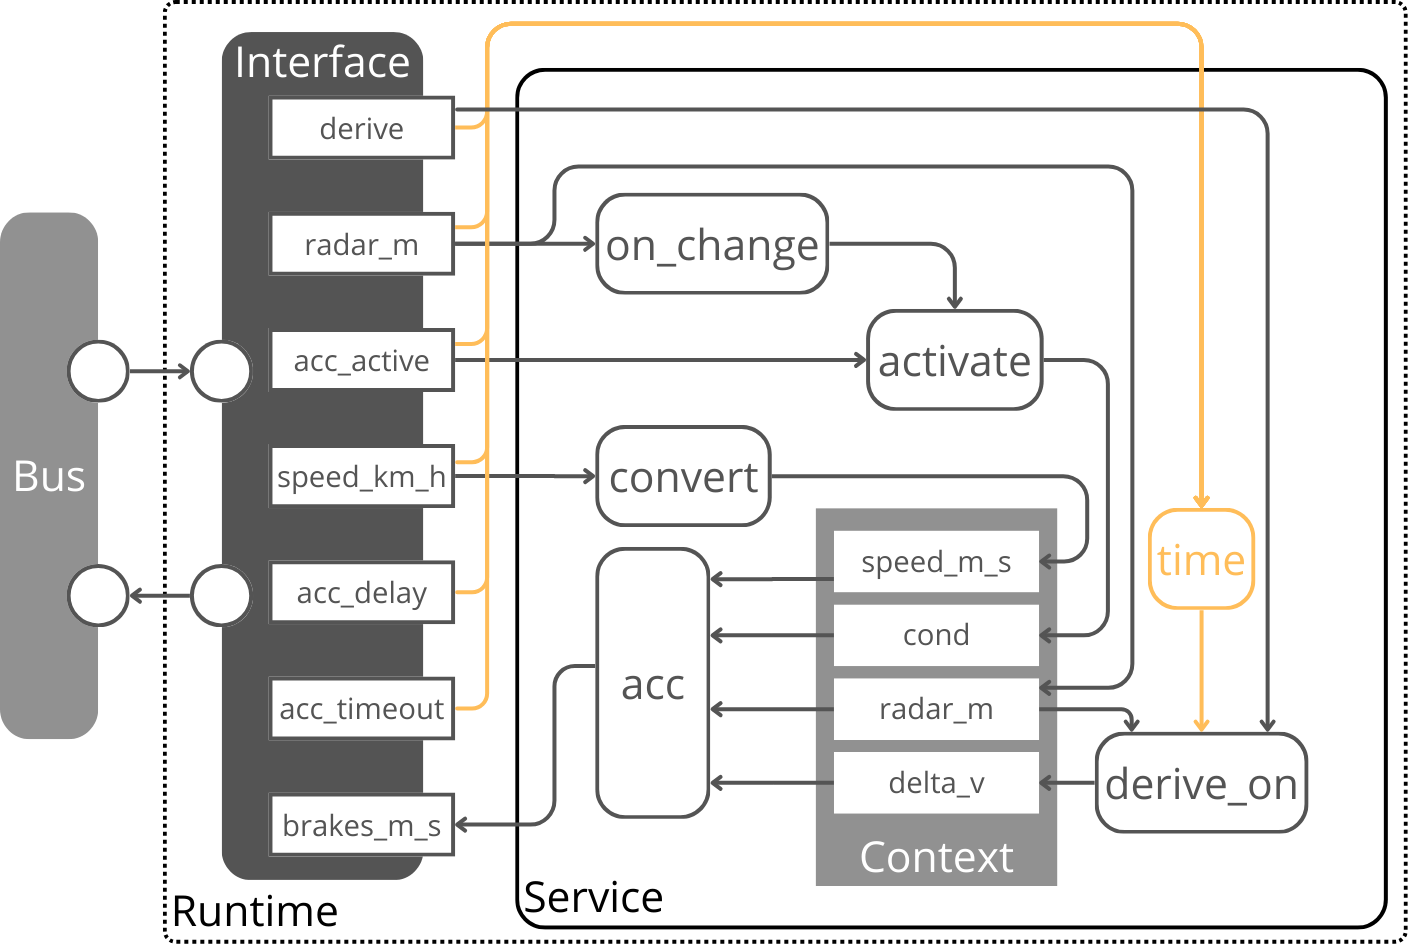
\includegraphics[width=0.7\textwidth]{../images/execution_acc.png}
  \caption[Adaptive Cruise Control execution.]%
  {Execution schematic for the Adaptive Cruise Control service from
    \Cref{fig:code_acc}.}
  \label{fig:execution_acc}
\end{figure}

Here is an example of propagation.
When \texttt{speed\_km\_h} changes, it triggers the \texttt{convert} component, which
updates \texttt{speed\_m\_s} in the context. Concurrently, the timestamp updates the
\texttt{time()} signal, which in turn triggers \texttt{derive\_on}. The
\texttt{derive\_on} component retrieves the value of the signal \texttt{radar\_m} from
the context and computes the updated value of \texttt{delta\_v}. Once
\texttt{speed\_m\_s} and \texttt{delta\_v} are updated, they propagate to the
\texttt{acc} component, ensuring that all its inputs are up to date. If one of its
inputs has changed, the \texttt{acc} component then computes the current value of
\texttt{brakes\_m\_s}. Finally, the value of \texttt{brakes\_m\_s} is sent through the
bus, only if it has changed.

To prevent both excessive updates and long periods without output, the service adheres
to timing constraints specified by \texttt{@[10, 3000]}
(\Cref{line:grust:example:acc_service:begin}). This annotation ensures that outputs are
produced at most every 10~ms and at least every 3000~ms. If inputs arrive faster than
the 10~ms minimum delay, they are buffered. These timing events are represented in
\Cref{fig:execution_acc} as \texttt{acc\_delay} and \texttt{acc\_timeout}. The
buffering mechanism is omitted from the diagram for clarity.


\begin{table}[ht!]
  \centering
  \begin{tabular}{l|ccccccccc}
    timestamp                 & {$t$}                 & {$t + 5$}      & {$t + 10$}         & {$t + 25$}         & {$t + 40$}         & {$t + 525$}         & {$t + 650$}         \\ \hline
    \verb|speed_km_h|         & 129.                  & \changed{131.} & \stored{131.}      & 131.               & 131.               & 131.                & \changed{128.}      \\
    \verb|radar_m|            & 130.                  & 130.           & 130.               & 130.               & \changed{125.}     & 125.                & 125.                \\
    \verb|acc_active|         & \changed{\texttt{On}} &                &                    &                    &                    &                     &                     \\
    \verb|derive|             &                       &                &                    & \changed{()}       &                    & \changed{()}        &                     \\
    \local{\texttt{x\_mem}}   & \local{130.}          & \local{$\bot$} & \local{130.}       & \local{130.}       & \local{130.}       & \local{125.}        & \local{125.}        \\
    \verb|time|               & \updated{$t$}         & $t$            & \updated{$t + 10$} & \updated{$t + 25$} & \updated{$t + 40$} & \updated{$t + 525$} & \updated{$t + 650$} \\
    \verb|delta_v|            & 0.                    & 0.             & 0.                 & 0.                 & 0.                 & \updated{-10.}      & -10                 \\
    \verb|radar_e|            &                       &                &                    &                    & \updated{125.}     &                     &                     \\
    \local{\texttt{active}}   & \local{true}          & \local{$\bot$} & \local{$\bot$}     & \local{$\bot$}     & \local{true}       & \local{$\bot$}      & \local{$\bot$}      \\
    \local{\texttt{r\_mem}}   & \local{130.}          & \local{$\bot$} & \local{$\bot$}     & \local{$\bot$}     & \local{125.}       & \local{$\bot$}      & \local{$\bot$}      \\
    \local{\texttt{approach}} & \local{false}         & \local{$\bot$} & \local{$\bot$}     & \local{$\bot$}     & \local{true}       & \local{$\bot$}      & \local{$\bot$}      \\
    \verb|cond|               & false                 & false          & false              & false              & \updated{true}     & true                & true                \\
    \verb|speed_m_s|          & 35.8                  & 35.8           & \updated{36.4}     & 36.4               & 36.4               & 36.4                & \updated{35.6}      \\
    \local{\texttt{fv\_v}}    & \local{$\bot$}        & \local{$\bot$} & \local{0.}         & \local{$\bot$}     & \local{36.4}       & \local{26.4}        & \local{25.6}        \\
    \local{\texttt{d\_safe}}  & \local{$\bot$}        & \local{$\bot$} & \local{0.}         & \local{$\bot$}     & \local{36.4}       & \local{89.7}        & \local{87.5}        \\
    \verb|brakes_m_s|         & 0.                    & 0.             & 0.                 & 0.                 & 0.                 & \updated{1.4}       & \updated{1.3}
  \end{tabular}
  \caption[Chronogram of an execution for the Adaptive Cruise Control.]%
  {Example chronogram for an execution of the ACC service from \Cref{fig:code_acc}.
    The legend for colors is: \changed{red} for input changes, \stored{green} for stored
    inputs, and \updated{blue} for local/exported flow updates. Internal component
    variables are in \local{gray}; \local{$\bot$} denotes absence of a value.
  }
  \label{fig:chronogram_acc}
\end{table}

\Cref{fig:chronogram_acc} shows an execution trace of the ACC service, which we can
follow step by step:
\begin{itemize}
  \item At time $t$, the driver activates the ACC, causing the \texttt{acc\_active} event to
        occur with the value \texttt{On}. This triggers the \texttt{activate} component, where
        the \texttt{act?} branch (\Cref{line:grust:example:when:act}) sets the internal state
        \texttt{active} to \texttt{true}. However, the \texttt{approach} state remains
        \texttt{false}, so the activation condition \texttt{cond} is \texttt{false}.
        Consequently, the output \texttt{brakes\_m\_s} remains at its initial value of 0.

  \item At $t+5$, a change in \texttt{speed\_km\_h} arrives. However, because the 10~ms minimum
        delay specified by \texttt{@[10, 3000]} (\Cref{line:grust:example:acc_service:begin})
        has not elapsed, the update is buffered and computation is deferred.

  \item At $t+10$, the minimum delay has passed, and the buffered input is processed. This
        triggers the \texttt{convert} component, updating \texttt{speed\_m\_s}. This change
        propagates to the \texttt{acc} component, but since \texttt{cond} is still
        \texttt{false}, the component's \texttt{match} statement
        (\Cref{line:grust:example:acc:begin}) takes the \texttt{false} branch, setting the
        braking force to 0 and leaving the output unchanged.

  \item At $t+25$, the \texttt{derive} event occurs, triggering the \texttt{derive\_on}
        component. Although a computation occurs, the resulting \texttt{delta\_v} is 0, so the
        output of \texttt{acc} remains unchanged.

  \item At $t+40$, the \texttt{radar\_m} signal changes from 130 to 125. This triggers the
        \texttt{on\_change} operator (\Cref{line:grust:example:on_change}), which emits the
        \texttt{radar\_e} event. In the \texttt{activate} component, the \texttt{r?} branch
        (\Cref{line:grust:example:declaration}) executes. Since the new radar value (125) is
        less than the previously stored one (130), the \texttt{approach} state becomes
        \texttt{true}. With both \texttt{active} and \texttt{approach} now being \texttt{true},
        the output \texttt{cond} becomes \texttt{true}. Although \texttt{acc} is now active,
        the braking force is still computed as zero because its input \texttt{delta\_v} is
        zero, so no new value is sent to the bus.

  \item At $t+525$, another \texttt{derive} event triggers \texttt{derive\_on}
        (\Cref{line:grust:example:derive_on:begin}). This time, using the previous radar and
        time values, \texttt{delta\_v} is updated to $-10$. This significant change in one of
        the inputs to \texttt{acc} causes it to recompute the braking force. With a non-zero
        relative speed, the \texttt{true} branch of the \texttt{match} statement now yields a
        braking force of $0.60$, which is sent to the bus.

  \item Finally, at $t+650$, a change in \texttt{speed\_km\_h} updates \texttt{speed\_m\_s}.
        This change again triggers the \texttt{acc} component, which re-evaluates its logic
        and outputs a new braking force of $0.57$.
\end{itemize}

\subsection{Verification}
\label{sec:grust:example:greusot}

The \iso standard governs functional safety for automotive systems, defining Automotive Safety
Integrity Levels (\Asil) from A (least critical) to D (most critical). Achieving compliance for
critical systems (\Asil~D) requires rigorous verification to prove the absence of faults like
arithmetic overflows or memory errors. Since runtime checks are often too costly for embedded
environments, this proof is typically done through static verification.

For an engineer, formal verification of traditional \Ci code imposes a significant burden. They must
manually prove fundamental memory safety properties, such as the absence of null pointer
dereferences, buffer overflows, or data races. This process is tedious and error-prone, consuming
effort that could be spent on verifying the functional logic of the system itself. In contrast,
\GRust generates \Rust code, a language whose design offers a distinct advantage for verification.
The \Rust compiler's borrow checker statically enforces memory and thread safety, eliminating entire
classes of bugs before the formal verification stage even begins.

This foundation allows a deductive verifier like \Creusot~ \cite{DBLP:conf/icfem/DenisJM22} to
streamline the proof process. From the user's perspective, the task shifts from proving low-level
memory correctness to specifying and proving high-level functional properties. An engineer annotates
their code with contracts---preconditions, postconditions, and invariants---that capture the
intended behavior. Verification is then performed by running \texttt{cargo creusot prove} on the
crate containing the generated code. \Creusot then attempts to prove that the implementation adheres
to these contracts.
%
By default, it also proves the absence of runtime panics, such as arithmetic overflows, providing a
strong baseline of safety automatically. For more advanced needs, engineers can add explicit
properties to verify critical system logic. To make these capabilities accessible at the modeling
level, we introduce \GReusot, a wrapper for the specification language of \Creusot that enables
verification of \GRSync components and functions.

\subsubsection{Specifying the ACC in \GReusot}
\label{sec:grust:example:greusot:acc}

\Cref{lst:grust:example:greusot:fun:spec,lst:grust:example:greusot:comp:spec} show the ACC example
extended with \GReusot specifications. Since \Creusot does not support
floating-point arithmetic, all values are represented as integers.

The specification for the \texttt{safety\_distance} function, shown in
\Cref{lst:grust:example:greusot:fun:spec}, defines its expected operating conditions. The
preconditions, specified in
\Cref{line:grust:example:greusot:fun:spec:sv_v,line:grust:example:greusot:fun:spec:fv_v}, state that
the subject vehicle speed (\texttt{sv\_v}) must be positive and at most 50 m/s, while
the front vehicle speed (\texttt{fv\_v}) must be slower, with a speed difference of no
more than 10 m/s. Under these assumptions, the postcondition in
\Cref{line:grust:example:greusot:fun:spec:result} guarantees that the computed safety
distance (\texttt{result}) is always positive and less than 150 meters (the maximum
radar range), while also ensuring the computation is free of overflows.

\begin{lstlisting}[
      label=lst:grust:example:greusot:fun:spec,
      language=GRust, 
      caption={[\GReusot specification of a function.]%
      \GReusot specification of the \texttt{safety\_distance} function from 
      \Cref{fig:code_acc}.},
      captionpos=b
]
function safety_distance(sv_v: int, fv_v: int) -> int
  requires { 0 < sv_v && sv_v <= 50 } $\label{line:grust:example:greusot:fun:spec:sv_v}$
  requires { 0 < fv_v && fv_v < sv_v && sv_v - fv_v <= 10 } $\label{line:grust:example:greusot:fun:spec:fv_v}$
  ensures  { 0 < result && result < 150 } $\label{line:grust:example:greusot:fun:spec:result}$
{
  let (rho: int, b_max: int) = (1, 6);
  let sv_d_stop: int = sv_v*rho + sv_v^2/(2*b_max);
  let fv_d_stop: int = fv_v^2/(2*b_max);
  return sv_d_stop - fv_d_stop;
}
\end{lstlisting}

The specification for the \texttt{acc} component (\Cref{lst:grust:example:greusot:comp:spec})
also defines several preconditions. First, it assumes in
\Cref{line:grust:example:greusot:comp:spec:d} that the radar distance \texttt{d} is always
between 0 and 150 meters. It then specifies, in the range
\Crefrange{line:grust:example:greusot:comp:spec:c:begin}{line:grust:example:greusot:comp:spec:c:end},
conditions that must hold whenever the ACC is active (\ie when \texttt{c} is true).
These require that the vehicle speed is within the valid range, that the vehicles are
approaching (relative speed \texttt{v} is negative), and that the distance between
them provides a sufficient margin for braking. This last condition prevents division
by zero in the braking computation. The postcondition in
\Cref{line:grust:example:greusot:comp:spec:b} guarantees that the computed braking rate
\texttt{b} remains within a safe interval (0 to 6 m/s²) and that no overflow and division by zero
occurs.
Proving this specification requires an auxiliary function, \texttt{compute\_braking}
(\Crefrange{line:grust:example:greusot:comp:spec:aux:begin}{line:grust:example:greusot:comp:spec:aux:end}),
to guide the solver.

This need to guide the solver highlights a practical aspect of formal verification.
Achieving certification for complex systems is rarely a fully automated process. It
demands expertise from a verification engineer, who must understand the strengths and
weaknesses of the underlying automated solvers. These solvers often struggle with
certain mathematical constructs, such as the non-linear arithmetic present in this
example (\texttt{v\^{}2}). The engineer must then provide intermediate lemmas or decompose
the proof, as done here with \texttt{compute\_braking}, to make the problem tractable
for the tool. This human-in-the-loop approach is a crucial part of applying formal
methods successfully to meet rigorous industrial standards.

\begin{lstlisting}[
  label=lst:grust:example:greusot:comp:spec,
  language=GRust, 
  caption={[\GReusot specification of a component.]%
  \GReusot specification of the \texttt{acc} component from \Cref{fig:code_acc}.},
  captionpos=b
]
component acc(c: bool, d: int, s: int, v: int) -> (b: int)
  // radar detection limitation
  requires { 0 < d && d < 150 } $\label{line:grust:example:greusot:comp:spec:d}$
  // ACC scope of usage
  requires { c => (0 < s && s <= 50) && (0 < s+v && v < 0 && -v <= 10) } $\label{line:grust:example:greusot:comp:spec:c:begin}$
  // there is enough distance to brake at maximum rate
  requires { c => d - safety_distance(s, s+v) > (v^2)/12 } $\label{line:grust:example:greusot:comp:spec:c:end}$
  // braking rate is in correct interval
  ensures  { 0 <= b && b <= 6 } $\label{line:grust:example:greusot:comp:spec:b}$
{
  match c {
    true => {
      b = compute_braking(d - d_safe, v);
      let d_safe: int = safety_distance(s, fv_v);
      let fv_v: int = s + v;
    }
    false => {
      b = 0;
      let (fv_v: int, d_safe: int) = (0, 0);
    }
  }
}
// Intermediate braking function to pass the proof
function compute_braking(d_grace: int, v: int) -> int $\label{line:grust:example:greusot:comp:spec:aux:begin}$
  // scope
  requires { (0 < d_grace &&  d_grace < 150) && (v < 0 && -v <= 10) }
  // there is enough distance to brake at maximum rate
  requires { d_grace > (v^2)/12 }
  // braking rate is in correct interval
  ensures  { 0 <= result && result <= 6 }
{
  return (v^2) / (2*d_grace);
} $\label{line:grust:example:greusot:comp:spec:aux:end}$
\end{lstlisting}

\subsection{Summary}
This section used an Adaptive Cruise Control system to illustrate the core features of \GRust. The
example showed how the language combines the asynchronous, dataflow-oriented \GRFRP kernel for
service modeling with the synchronous, equation-based \GRSync kernel for defining reusable
components. The execution trace highlighted the efficiency of the event-driven model, where
computations are performed only in response to relevant input changes. Finally, the integration with
\GReusot demonstrated how safety-critical properties can be specified and formally verified at the
modeling level, leveraging the inherent safety of the generated \Rust code. Together, these elements
show how \GRust provides a cohesive framework for designing, implementing, and verifying complex
reactive systems in a way that is expressive for engineers, compatible with  in \sdv architecture
and suitable for safety-critical applications.
